\documentclass{beamer}
\usepackage{mathtools}
\usepackage{pgfplots}
\pgfplotsset{compat=newest}
\usetheme{CambridgeUS}  % Select your favorite theme


\title{The geometry of blowups}
\author{Further material}
\institute{Complex Singularities}
\date{\today}

\begin{document}




\begin{frame}
\titlepage
\end{frame}


\begin{frame}
\frametitle{Introduction}

The blowup is the most simple and typical case of a birational map\footnote{a rational map such that its inverse is also rational} that is not an isomorphism.\newline It is the typical method of \textit{resolving singularities}.

\begin{center}
    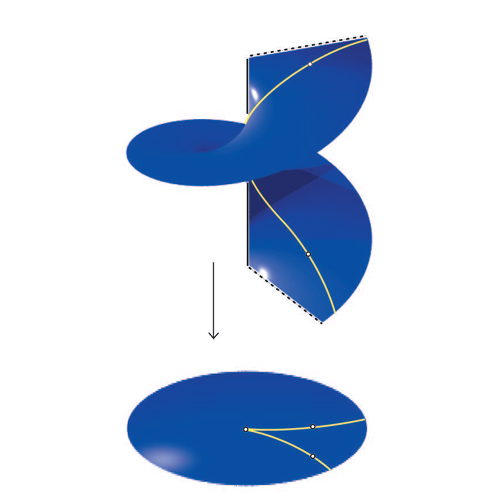
\includegraphics[scale=0.3]{1.PNG}
\end{center}

\end{frame}
\begin{frame}
\frametitle{Resolution of singularities}
Suppose $X$ is an algebraic set with singularities. We want to find a manifold $X^\prime$ such that there exists a map $\pi : X^\prime \to X$ which parametrizes $X$. For example, recall the difference between \textit{regular surfaces} and \textit{parametrized surfaces}.\newline\newline This is called \textbf{resolving singularities}.
\end{frame}
\begin{frame}
\frametitle{Some examples of resolutions}
\begin{example}
    Consider the cylinder $x^2 + y^2 = 1$ in $\mathbb{A}^3$, and the map from this cylinder to $X = \{(x,y,z) \in \mathbb{A}^3 \mid x^2 + y^2 - z^2 = 0\}$ given by \[\pi: (x,y,z) \mapsto (xz,yz,z)\] In this case, we already knew $X^\prime$. However, in further examples we try to construct resolutions. The main technique is \textbf{blowing up} points.
\end{example}
\end{frame}

\begin{frame}
\frametitle{Blowing up the singularity of $y^2 = x^3 + x^2$}

Substituting $y = tx$, we get the equation $x^2(t^2-(x+1)) = 0$ which yields two nonsingular curves.

\phantom{?}

\begin{minipage}{.5\textwidth}
    \scalebox{0.7}{
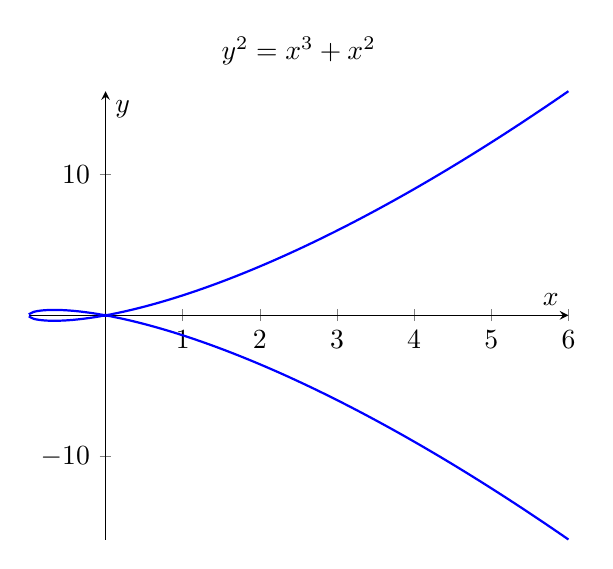
\begin{tikzpicture}
  \begin{axis}[
    axis lines = middle,
    xlabel = $x$,
    ylabel = $y$,
    domain=-6:6,
    samples=200,
    clip=false,
    title={$y^2 = x^3 + x^2$}
    ]
    \addplot[blue, thick, smooth] {sqrt(x^3+x^2)};
    \addplot[blue, thick, smooth] {-sqrt(x^3+x^2)};

  \end{axis}
\end{tikzpicture}}
\end{minipage}%
\begin{minipage}{.5\textwidth}
    \scalebox{0.7}{
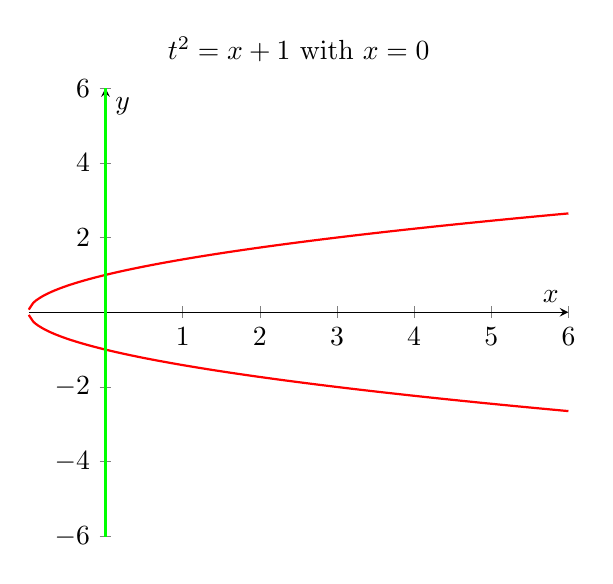
\begin{tikzpicture}
  \begin{axis}[
    axis lines = middle,
    xlabel = $x$,
    ylabel = $y$,
    domain=-6:6,
    samples=200,
    clip=false,
    title={$t^2 = x + 1$ with $x=0$}
    ]
    \addplot[red, thick, smooth] {sqrt(x+1)};
    \addplot[red, thick, smooth] {-sqrt(x+1)};
    \addplot[green, thick, smooth] (0,x);
  \end{axis}
\end{tikzpicture}}
\end{minipage}

\end{frame}

\begin{frame}
\frametitle{Blowing up the singularity of $y^2 = x^3 + x^2$}

In this case, the singularity $(0,0)$ is considered to be replaced with the line $x=0$, or equivalently all directions in the line passing through $(0,0)$.
\pause\newline
We call the line $x= 0$ the \textbf{exceptional curve}.

\end{frame}
\begin{frame}
\frametitle{Blowing up points in higher dimensions}
\begin{example}
    Consider the cone $x^2 + y^2 = z^2$ in $\mathbb{A}^3$. This has a singularity at $O$, so we try to resolve it by substituting $x = zs$ and $y = zt$. We get $ z^2(s^2+t^2-1)=0$, which again leads to two nonsingular varieties. We call $z=0$ the exceptional plane.
\end{example}
\end{frame}


\begin{frame}
\frametitle{Singular varieties that need more than one blowup to resolve them}
\begin{example}
    Consider the curve $y^8 = z^5$ in $\mathbb{A}^2$. Let $z = yt$ to get $y^5(t^5-y^3)=0$. This is not yet nonsingular. Therefore, we take $t^5 - y^3 = 0$ and blow it up again. Let $y = ts$, to get $t^3(s^3-t^2) = 0$. Blow up one more time to get nonsingular varieties.
\end{example}
\end{frame}

\begin{frame}
\frametitle{Formal definition}
I could not find a suitable formal definition of a blowup of general spaces...
\end{frame}


\section{A special definition}

\begin{frame}
\frametitle{Blowups of projective spaces}

Consider $\mathbb{P}^n$ and $\mathbb{P}^{n-1}$ with coordinates $(x_0 : \cdots : x_n)$ and $(y_1: \cdots :y_n)$ respectively. For points $x = (x_0 : \cdots : x_n)$ and $y = (y_1 : \cdots : y_n)$, denote $(x,y) \in \mathbb{P}^n \times \mathbb{P}^{n-1}$ as $(x_0 : \cdots :x_n : y_1 : \cdots : y_n)$.\pause

Consider the closed subvariety $\Pi \subset \mathbb{P}^n\times \mathbb{P}^{n-1}$ defined by \[\{(x,y)\in\mathbb{P}^n\times\mathbb{P}^{n-1} \mid x_iy_j = x_jy_i \quad \text{for} \quad i,j = 1,\ldots,n\}\]

\end{frame}


\begin{frame}
\frametitle{Blowups of projective spaces}

\begin{definition}
    The map $\sigma: \Pi \to \mathbb{P}^n$ defined by restricting the first projection $\mathbb{P}^n\times \mathbb{P}^{n-1} \to \mathbb{P}^n$ is called the \textbf{blowup} of $\mathbb{P}^n$ centered at $\xi = (1:0:\cdots:0) \in \mathbb{P}^n$.
\end{definition}
\end{frame}


\begin{frame}
\frametitle{An exercise of the text}
\begin{problem}
    Prove that the blowup of the complex manifold $M$ at a point $m$ is diffeomorphic in an orientation preserving manner to the connected sum \[M\#\overline{\mathbb{P}}^N\] where $\overline{\mathbb{P}}^N$ is the oriented smooth manifold obtained by changing the canonical orientation of $\mathbb{P}^N$.
\end{problem}
\end{frame}



\end{document}
